
\subsection{Delay public release} \label{sec:3delay}

The best approach here is to keep the embargoed data on a secure device separate from other systems and migrate images to the regular repository as they become \emph{public}.
This can be an object store with encryption like MinIO \footnote{\url{ https://min.io/product/enterprise-object-storage-encryption}}.
We will need to have one at SLAC and one at Chile for redundancy to ensure no data loss.

With the commissioning constraint that means this needs to be a 30 day store  for full images and engineering data.
Looking at \citeds{DMTN-135}
table 40 this comes out to about 500TB of usable disk.
\tabref{tab:delay} gives the cost calculation or this.

The nominal embargo for regular operations we understand as between 80 hours (most images) and 10 days (some images as specified by Alert Vetting).

\tiny \begin{longtable} {|p{0.3\textwidth}|r|l|} \caption{This table provides costs for the embargoed data store.  \label{tab:delay}}\\ 
\hline 
\textbf{Description}&\textbf{value}& \\ \hline
{Number of days data to store}&{30}& \\ \hline
{Raw data size per day (TB compressed)}&{16}&{Years data from Table 40 of \citeds{DMTN-135}\/ 298.3 observing nights (Key Numbers Confluence) } \\ \hline
{Useable size needed (TB)}&{484}& \\ \hline
{Allowing for RAID (TB)}&{1000}& \\ \hline
{Cost for 1 store}&{\$400,000}&{Using SLAC Fast Disk Price from Table 28 of \citeds{DMTN-135}} \\ \hline
\textbf{Total for 2 stores}&\textbf{\$800,000}& \\ \hline
{Ops Cost at least 1 Refresh}&{\$800,000}& \\ \hline
\end{longtable} \normalsize



{\bf Note:} If we assume the security requirements apply to commissioning i.e. we must use encrypted storage and encrypted lines, then we can not carry out commissioning activities at NCSA. This implies SLAC must be ready for ComCam.

\figref{fig:arch} depicts the encrypted storage and network. Embargoed (delayed) data would be held in the encrypted stores for the time specified.
We assume temporary processing for alerts does not have to be encrypted, NIST allows ephemeral unencrypted data for processing.

\begin{figure}
\begin{centering}
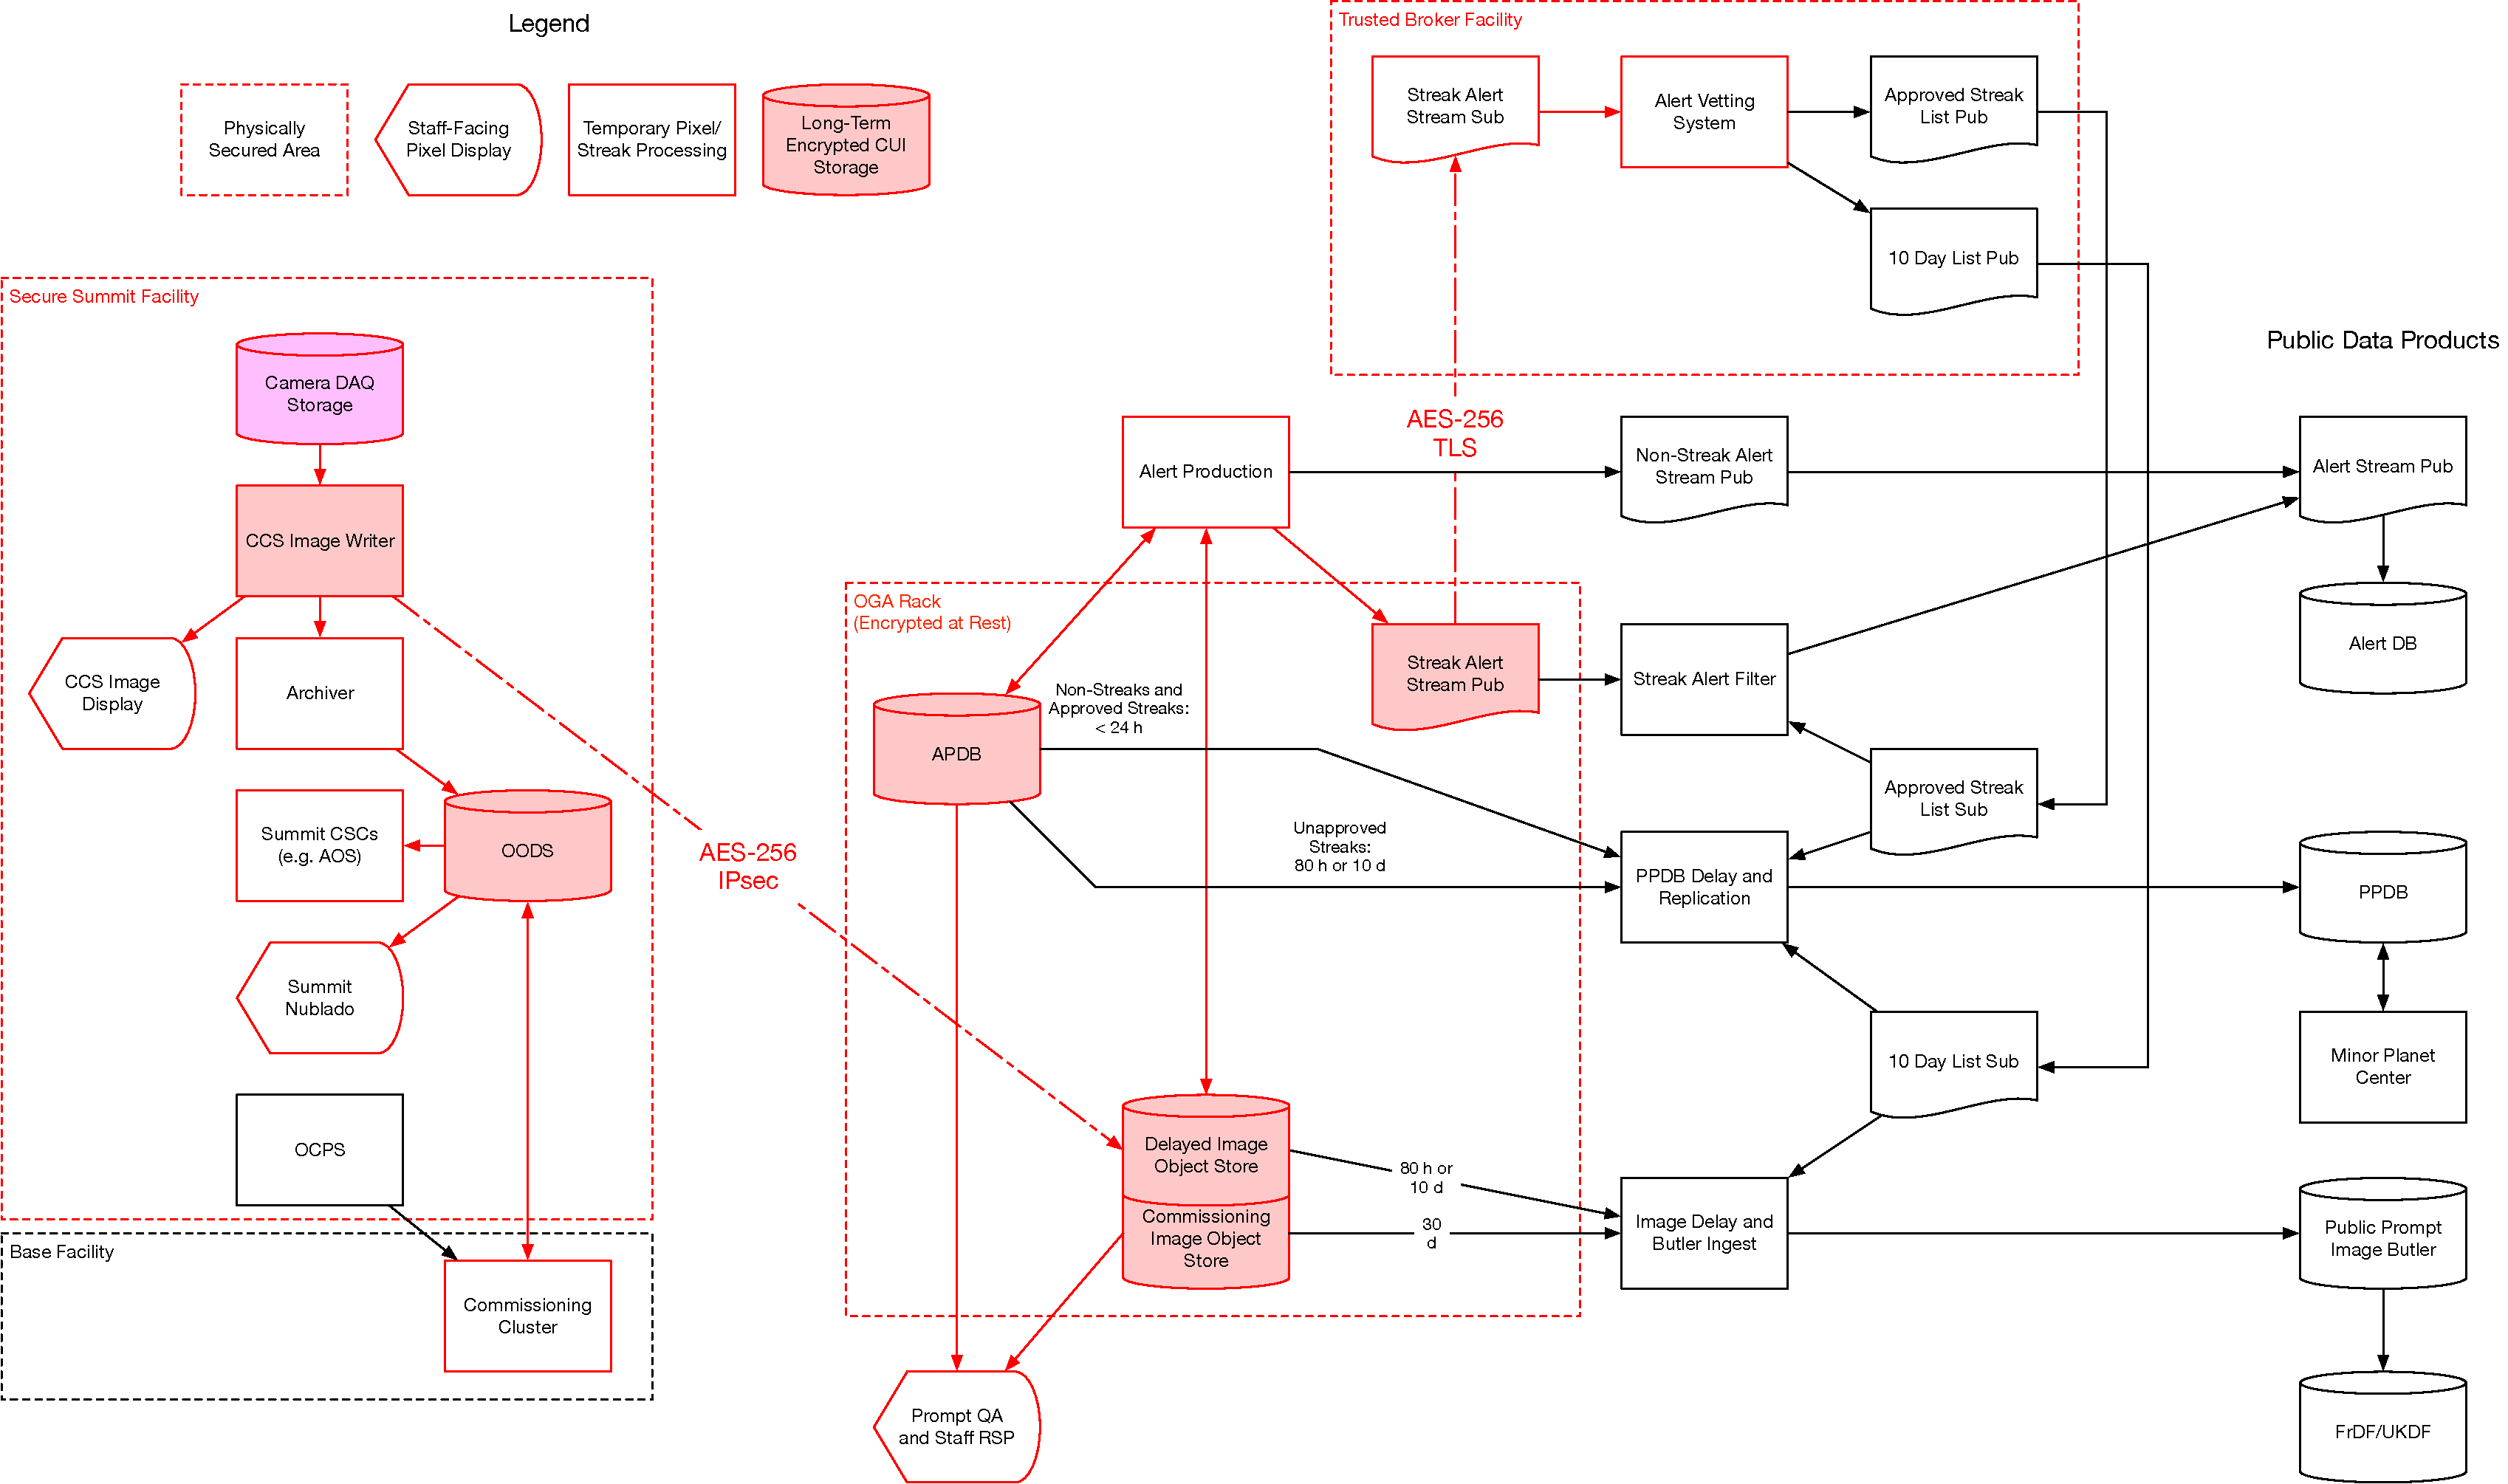
\includegraphics[width=\textwidth]{OGA_Diagram}
	\caption{ OGA architecture  showing the long term encrypted storage and encrypted network from Chile to SLAC. \label{fig:arch}}
\end{centering}
\end{figure}
